\documentclass[aap]{imsart}

%% Packages
\RequirePackage{amsthm,amsmath,amsfonts,amssymb}
\RequirePackage[numbers]{natbib}
%\RequirePackage[authoryear]{natbib} %% uncomment this for author-year bibliography
\RequirePackage[colorlinks,citecolor=blue,urlcolor=blue]{hyperref}
\RequirePackage{graphicx}
\usepackage{subcaption}


\startlocaldefs

\newcommand\var[1]{\, \mathrm{Var} \left( #1 \right)}

\newcommand\pr[1]{\, \mathbb{P} \left\lbrace #1 \right\rbrace}

\newcommand\cov[1]{\, \mathrm{Cov} \left( #1 \right)}

\newcommand\expec[1]{\, \mathbb{E} \left\lbrack #1 \right\rbrack}

\renewcommand{\S}{\textsf{S}}

\newcommand{\I}{\textsf{I}}

\newcommand{\R}{\textsf{R}}
 
%%%%%%%%%%%%%%%%%%%%%%%%%%%%%%%%%%%%%%%%%%%%%%
%%                                          %%
%% Uncomment next line to change            %%
%% the type of equation numbering           %%
%%                                          %%
%%%%%%%%%%%%%%%%%%%%%%%%%%%%%%%%%%%%%%%%%%%%%%
%\numberwithin{equation}{section}
%%%%%%%%%%%%%%%%%%%%%%%%%%%%%%%%%%%%%%%%%%%%%%
%%                                          %%
%% For Axiom, Claim, Corollary, Hypothezis, %%
%% Lemma, Theorem, Proposition              %%
%% use \theoremstyle{plain}                 %%
%%                                          %%
%%%%%%%%%%%%%%%%%%%%%%%%%%%%%%%%%%%%%%%%%%%%%%
%\theoremstyle{plain}
\newtheorem{axiom}{Axiom}
\newtheorem{claim}[axiom]{Claim}
\newtheorem{theorem}{Theorem}[section]
\newtheorem{lemma}[theorem]{Lemma}
%%%%%%%%%%%%%%%%%%%%%%%%%%%%%%%%%%%%%%%%%%%%%%
%%                                          %%
%% For Assumption, Definition, Example,     %%
%% Notation, Property, Remark, Fact         %%
%% use \theoremstyle{remark}                %%
%%                                          %%
%%%%%%%%%%%%%%%%%%%%%%%%%%%%%%%%%%%%%%%%%%%%%%
\theoremstyle{remark}
\newtheorem{definition}[theorem]{Definition}
\newtheorem*{example}{Example}
\newtheorem*{fact}{Fact}
%%%%%%%%%%%%%%%%%%%%%%%%%%%%%%%%%%%%%%%%%%%%%%
%% Please put your definitions here:        %%
%%%%%%%%%%%%%%%%%%%%%%%%%%%%%%%%%%%%%%%%%%%%%%

\endlocaldefs

\begin{document}

\begin{frontmatter}
\title{Stochastic epidemic models}
%\title{A sample article title with some additional note\thanksref{t1}}
%\runtitle{A sample running head title}
%\thankstext{T1}{A sample additional note to the title.}

\begin{aug}
%%%%%%%%%%%%%%%%%%%%%%%%%%%%%%%%%%%%%%%%%%%%%%
%%Only one address is permitted per author. %%
%%Only division, organization and e-mail is %%
%%included in the address.                  %%
%%Additional information can be included in %%
%%the Acknowledgments section if necessary. %%
%%%%%%%%%%%%%%%%%%%%%%%%%%%%%%%%%%%%%%%%%%%%%%
\author[A]{\fnms{Gerardo} \snm{Palafox}\ead[label=e1]{gerardo.palafoxcstl@uanl.edu.mx}},
%%%%%%%%%%%%%%%%%%%%%%%%%%%%%%%%%%%%%%%%%%%%%%
%% Addresses                                %%
%%%%%%%%%%%%%%%%%%%%%%%%%%%%%%%%%%%%%%%%%%%%%%
\address[A]{Facultad de Ingenier\'ia Mec\'anica y El\'ectrica,
Universidad Aut\'onoma de Nuevo Le\'on,
\printead{e1}}

\end{aug}

\begin{abstract}
In this work, a stochastic model for the spread of infectious diseases is presented. Theoretical results and simulations are shown. Additionally, data from the ongoing pandemic caused by the SARS-CoV-2 virus is incorporated to discuss the implications of the model.
%%%%	
%The abstract should summarize the contents of the paper.
%It should be clear, descriptive, self-explanatory and not longer
%than 200 words. It should also be suitable for publication in
%abstracting services. Formulas should be used as sparingly as
%possible within the abstract. The abstract should not make
%reference to results, bibliography or formulas in the body
%of the paper---it should be self-contained.
%
%This is a sample input file.  Comparing it with the output it
%generates can show you how to produce a simple document of
%your own.
\end{abstract}

\begin{keyword}[class=MSC2020]
\kwd[Primary ]{60J05}
\kwd{60J27}
\kwd[; secondary ]{92D30}
\end{keyword}

\begin{keyword}
\kwd{Stochastic processes}
\kwd{Epidemics}
\end{keyword}

\end{frontmatter}
%%%%%%%%%%%%%%%%%%%%%%%%%%%%%%%%%%%%%%%%%%%%%%
%% Please use \tableofcontents for articles %%
%% with 50 pages and more                   %%
%%%%%%%%%%%%%%%%%%%%%%%%%%%%%%%%%%%%%%%%%%%%%%
%\tableofcontents

\section{Introduction}\label{sect:intro}
The goal of this work is to present one of the most common stochastic epidemic models, alongside computational simulations of this. The terminology and theoretical preliminaries for later sections are detailed in Section \ref{sect:prelim}. In Section \ref{sect:related_work}, related work is presented. Models and variations are later presented in Sections \ref{sect:reedfrost}, \ref{sect:standard_model} and \ref{sect:network}. Finally, data from the current COVID-19 pandemic, caused by the SARS-CoV-2 virus, is discussed in Section \ref{sect:covid}.

\section{Preliminaries}\label{sect:prelim}
The probability of an event $A$ will be denoted by $\pr{A}$. If $X$ is a random variable, the expected value of $X$ and its variance are denoted by $\expec{X}$ and $\var{X}$ respectively. A sequence of random variables $X_1, X_2, \dots$, converges in probability to a random variable $X$ if, for every $\varepsilon > 0$, 
\begin{equation}
\lim_{n \rightarrow \infty} \pr{|X_n - X| \geq \varepsilon } = 0 \; \text{ or, equivalently, } \; \lim_{n \rightarrow \infty} \pr{|X_n - X| < \varepsilon } = 1.
\end{equation}
A sequence of random variables $X_1, X_2, \dots,$ converges in distribution to a random variable $X$ if 
\begin{equation}
\lim_{n \rightarrow \infty} F_{X_n} (x) = F_X (x),
\end{equation}
at all points $x$ where $F_{X} (x)$ is continuous, where $F_X$ is the distribution of the random variable $X$. A stochastic process is a collection $\lbrace X(t) : t \in J\rbrace$ of random variables. Index $t$ is often interpreted as time, and $X(t)$ is referred to as the state of the process at time $t$. The set $J$ is called the index set of the process, and determines whether the process is discrete-time or continuous-time, depending on whether $J$ is countable or an interval of the real line. A Markov chain is a stochastic process where the random variables take a finite or countable number of possible values, and with the property that
\begin{equation}
	\pr{X_{n+1} = j \mid X_{n} = i, X_{n-1} = i_{n-1}, \dots, X_0 = i_0 } = \pr{X_{n+1} = j \mid X_n = i},
\end{equation}
for any such states $i_k$ and any $n > 0$. 

\subsection{Related Work}\label{sect:related_work}
The mathematical study of epidemics has been long studied, with early models focusing on specific diseases \citep{BERNOULLI_1760, Ross_1910}. More general studies have been performed since then, being \citet{Kermack_McKendrick_1927} some of the first in doing so, and \citet{Bailey_1975, Frauenthal_1980, Brauer_Castillo-Chavez-2012} more recently. This work will focus on models with stochastic components \citep{Andersson_Britton_2000, Britton_2010}, but deterministic models have also been studied \citep{Hethcote_2000}. Models where the disease spreads over a network have been studied thoroughly, both in their deterministic \citep{Mei_Mohagheghi_Zampieri_Bullo_2017} and stochastic \citep{Britton_2019, Trapman_Bootsma_2009} form. Agent-based simulations have also been used to model epidemics \citep{Hoertel_Blachier_Blanco_Olfson_Massetti_Rico_Limosin_Leleu_2020}.

\section{Reed-Frost model}\label{sect:reedfrost} One of the simplest stochastic models of disease spreading is the Reed-Frost model, which is included in this work for reference. This model is a discrete-time Markov chain, were an individual in a finite population is classified as susceptible, infected or removed; these are called SIR models. The model in Section \ref{sect:standard_model} is also an SIR model. At time $t$, there are $S_t$ individuals susceptible to infection, and $I_t$ currently infectious. The incubation period of the disease, as well as the recovery time, is assumed to occur between time jumps. That is, susceptible people exposed at time $t$ will be infectious at time $t+1$, and people infectious at time $t$ will be removed from the process at time $t+1$.  Any two individuals have a probability $p = 1-q$ of coming in contact at time $t$, with encounters being independent of each other. As such, the distribution of $S_{t+1}$ is binomial $\mathrm{Bin}(s, q^i)$. Observe that $I_{t+1} = S_t - S_{t+1}$, since in the step from $t$ to $t+1$, all the infectious from time $t$ are removed, and the decrease in susceptible individuals is precisely the amount of new infectious people. Thus, $I_{t+1} \sim \mathrm{Bin}(s, 1-q^i)$. More of this process and its asymptotic properties can be read in a work by \citet{VonBahr}.

\section{Standard stochastic epidemic model}\label{sect:standard_model}
The construction and details of this model can be found in the book of \citet{Andersson_Britton_2000}. A description of the properties presented in Subsection \ref{subs:properties}, among more, can be found in a survey by \citet{Britton_2010}. A fixed population of size $n$ will be considered. It is assumed there are no births, deaths or migration; this is what is known as a closed population. Additionally, population is assumed well-mixed and homogeneous: this means any two elements of the population can be in contact with each other, and everyone is affected by the disease in the same way. Each individual will be either susceptible (S), infectious (I), or recovered (R, also called removed). Let $S(t), I(t), R(t)$ be the number of susceptible, infectious and recovered individuals at time $t$. At $t = 0$, one has $S(0) = n - m, I(0) = m, R(0) = 0$. The contacts an infectious individual has with others follows a Poisson process with intensity $\lambda$ \citep{Andersson_Britton_2000, lawler_2006}. Each such contact is with an individual selected uniformly at random from the population, with contacts of different infectious individuals being mutually independent. When the contact occurs between an infectious individual and a susceptible individual, the susceptible individual is assumed to be infected, and it is immediately infectious. Every infectious individual remains so for a random time $I \sim F_I$, called the \textit{infectious period}, where $F_I$ has mean $1/\gamma$. These infectious periods are independent and identically distributed, and are independent from the contact process.  Epidemic starts at time 0, and goes until a time $T$ where $I(T) = 0$. Thus the final state of the epidemic is given by  $S(T) = n - R(T), I(T) = 0$ and $R(T) = m + Z$; i.e., $Z$ people where infected in the course of the epidemic. While, regardless of the distribution $F_I$, there is no closed form expression for the time dynamics of the process, it is possible to derive a recursive formula for the final size of the epidemic, see the survey of \citet{Britton_2010}. However, this becomes difficult for even moderately large $n$ \citep{Britton_2010}.

When $F_I \sim \mathrm{Exp}(\gamma)$, the model becomes a continuous-time Markov chain, known as the \textit{stochastic general epidemic model}, which was first considered by \citet{Bartlett_1949}. There is no epidemiological reason to assume the infectious period follows an exponential distribution, but doing so is of mathematical convenience, as it allows diffusion approximations valid for large values of $n$ \citep{Andersson_Britton_2000}. If the infectious period is not random but constant, the resulting model is a continuous-time version of the Reed-Frost model \citep{Andersson_Britton_2000} (see Section \ref{sect:reedfrost} for a definition of this model).

\subsection{Properties of the model}\label{subs:properties}
The aim of this section is to explore key questions revolving around an epidemic process, such as the probability of having a major outbreak, or how many people will be infected in such an outbreak. An approximation of the early stages of the epidemic process is also considered. Everything presented will be independent of the distribution $F_I$, i.e. it will not rely on the Markovian case.

\citet{Britton_2010} details how, when $n$ is sufficiently large, the initial phase of the epidemic can be approximated by a homogeneous branching process with birth-rate $\lambda$ and life-distribution $I \sim F_I$ \citep{lawler_2006} having Laplace transform $\phi(s)$. The epidemic and branching process will agree at least until there has been $k$ contacts, with $k$ small in relation to $\sqrt{n}$. The offspring distribution of the branching process has mean $\lambda \expec{I} = \lambda/\gamma$  \citep{Britton_2010}, a quantity denoted by $R_0$ from here on. Also mentioned by \citet{Britton_2010} is the fact that when $R_0 \leq 1$ the final size of the epidemic is bounded in probability, and it is not when $R_0 > 1$. Additionally, if $R_0 > 1$, the epidemic will be minor with probability $q^m$ and mayor with probability $\rho = 1-q^m$, where $q$ is the smallest solution to 
\begin{equation}\label{eq:q}
	q = \phi(\lambda (1-q)).
\end{equation}
A more detailed treatment of the properties just stated can be found in the work of \citet{Ball_1983}. The number $R_0$ is known in the literature as the \textit{basic reproduction number}, and, as it is seen, plays an important role in whether the epidemic dies out \textquotedblleft rapidly\textquotedblright or there is a major outbreak.

A rigorous study of the final size of the epidemic can be found in the work of \citet{Scalia-Tomba_1985, Scalia-Tomba_1990}. \citet{Britton_2010} gives a balance equation to find the fraction of people not getting infected. Particularly, one can find in his work \citep{Britton_2010} that if $z$ is the fraction of people infected, by the law of large numbers the limiting fraction infected in case of a major outbreak is a solution to the equation
\begin{equation}\label{eq:limiting_fraction}
	1-z = e^{-R_0 z}.
\end{equation}
The value $z = 0$, which corresponds to a minor outbreak, is always a solution to this equation. Also, when $R_0 > 1$, there exists an additional unique solution $z^\ast$ in the unit interval. Furthermore, denoting by $Z_n$ the final number of infected individuals for a population of size $n$, one has that if $R_0 \leq 1$, then $\bar{Z_n} := Z_n / n \rightarrow 0$ in probability as $n \rightarrow \infty$ \citep{Britton_2010}. If, however, $R_0 > 1$, then $\bar{Z_n} \rightarrow \zeta$, where $\zeta$ is a two point distribution defined by $\pr{\zeta = 0} = q^m, \pr{\zeta = z^\ast} = 1-q^m$ \citep{Britton_2010}, with $q$ as seen in Equation \ref{eq:q} and $z^\ast$ being the positive solution to Equation \ref{eq:limiting_fraction} previously mentioned. Defining $r^2 = \var{I} / (\expec{I})^2$, when $\bar{Z_n} \rightarrow z^\ast$ one has
\begin{equation}
	\sqrt{n} (\bar{Z_n} - z^\ast) \rightarrow \mathcal{N}\left(0, \frac{z^\ast (1-z^\ast)(1+r^2(1-z^\ast)R_{0}^{2}) }{(1-(1-z^\ast)R_{0})^2}\right),
\end{equation}
where $\mathcal{N}(\mu, \sigma^2)$ denotes a normal distribution of mean $\mu$ and variance $\sigma^2$.

\subsection{Simulations} \label{subs:simulation:}
The code for the simulations in this and further sections is publicly available in a GitHub repository\footnote{\url{https://github.com/palafox794/AppliedProbabilityModels/tree/master/FinalProject}}. The simulations were performed using Gillespie's direct method algorithm \citep{Drake_Rohani}. In Figure \ref{fig:trajectories}, two trajectories of the stochastic general epidemic model are shown. Both consist of a population of 1000 with 10 initial infected. The trajectory in Figure \ref{fig:trajectory_small_epidemic} has an $R_0 = .5$ and the one in Figure \ref{fig:trajectory_big_epidemic} has an $R_0 = 1.5$. In Figure \ref{fig:final_size}, final size distributions of these models are displayed; Figure \ref{fig:final_size_small_epidemic} shows the distribution of the final size of the model with $R_0 = .5$, while Figure \ref{fig:final_size_big_epidemic} shows the distribution of the final size of the model with $R_0 = 1.5$. 

\begin{figure}
	\centering
	\begin{subfigure}{0.45\linewidth}
		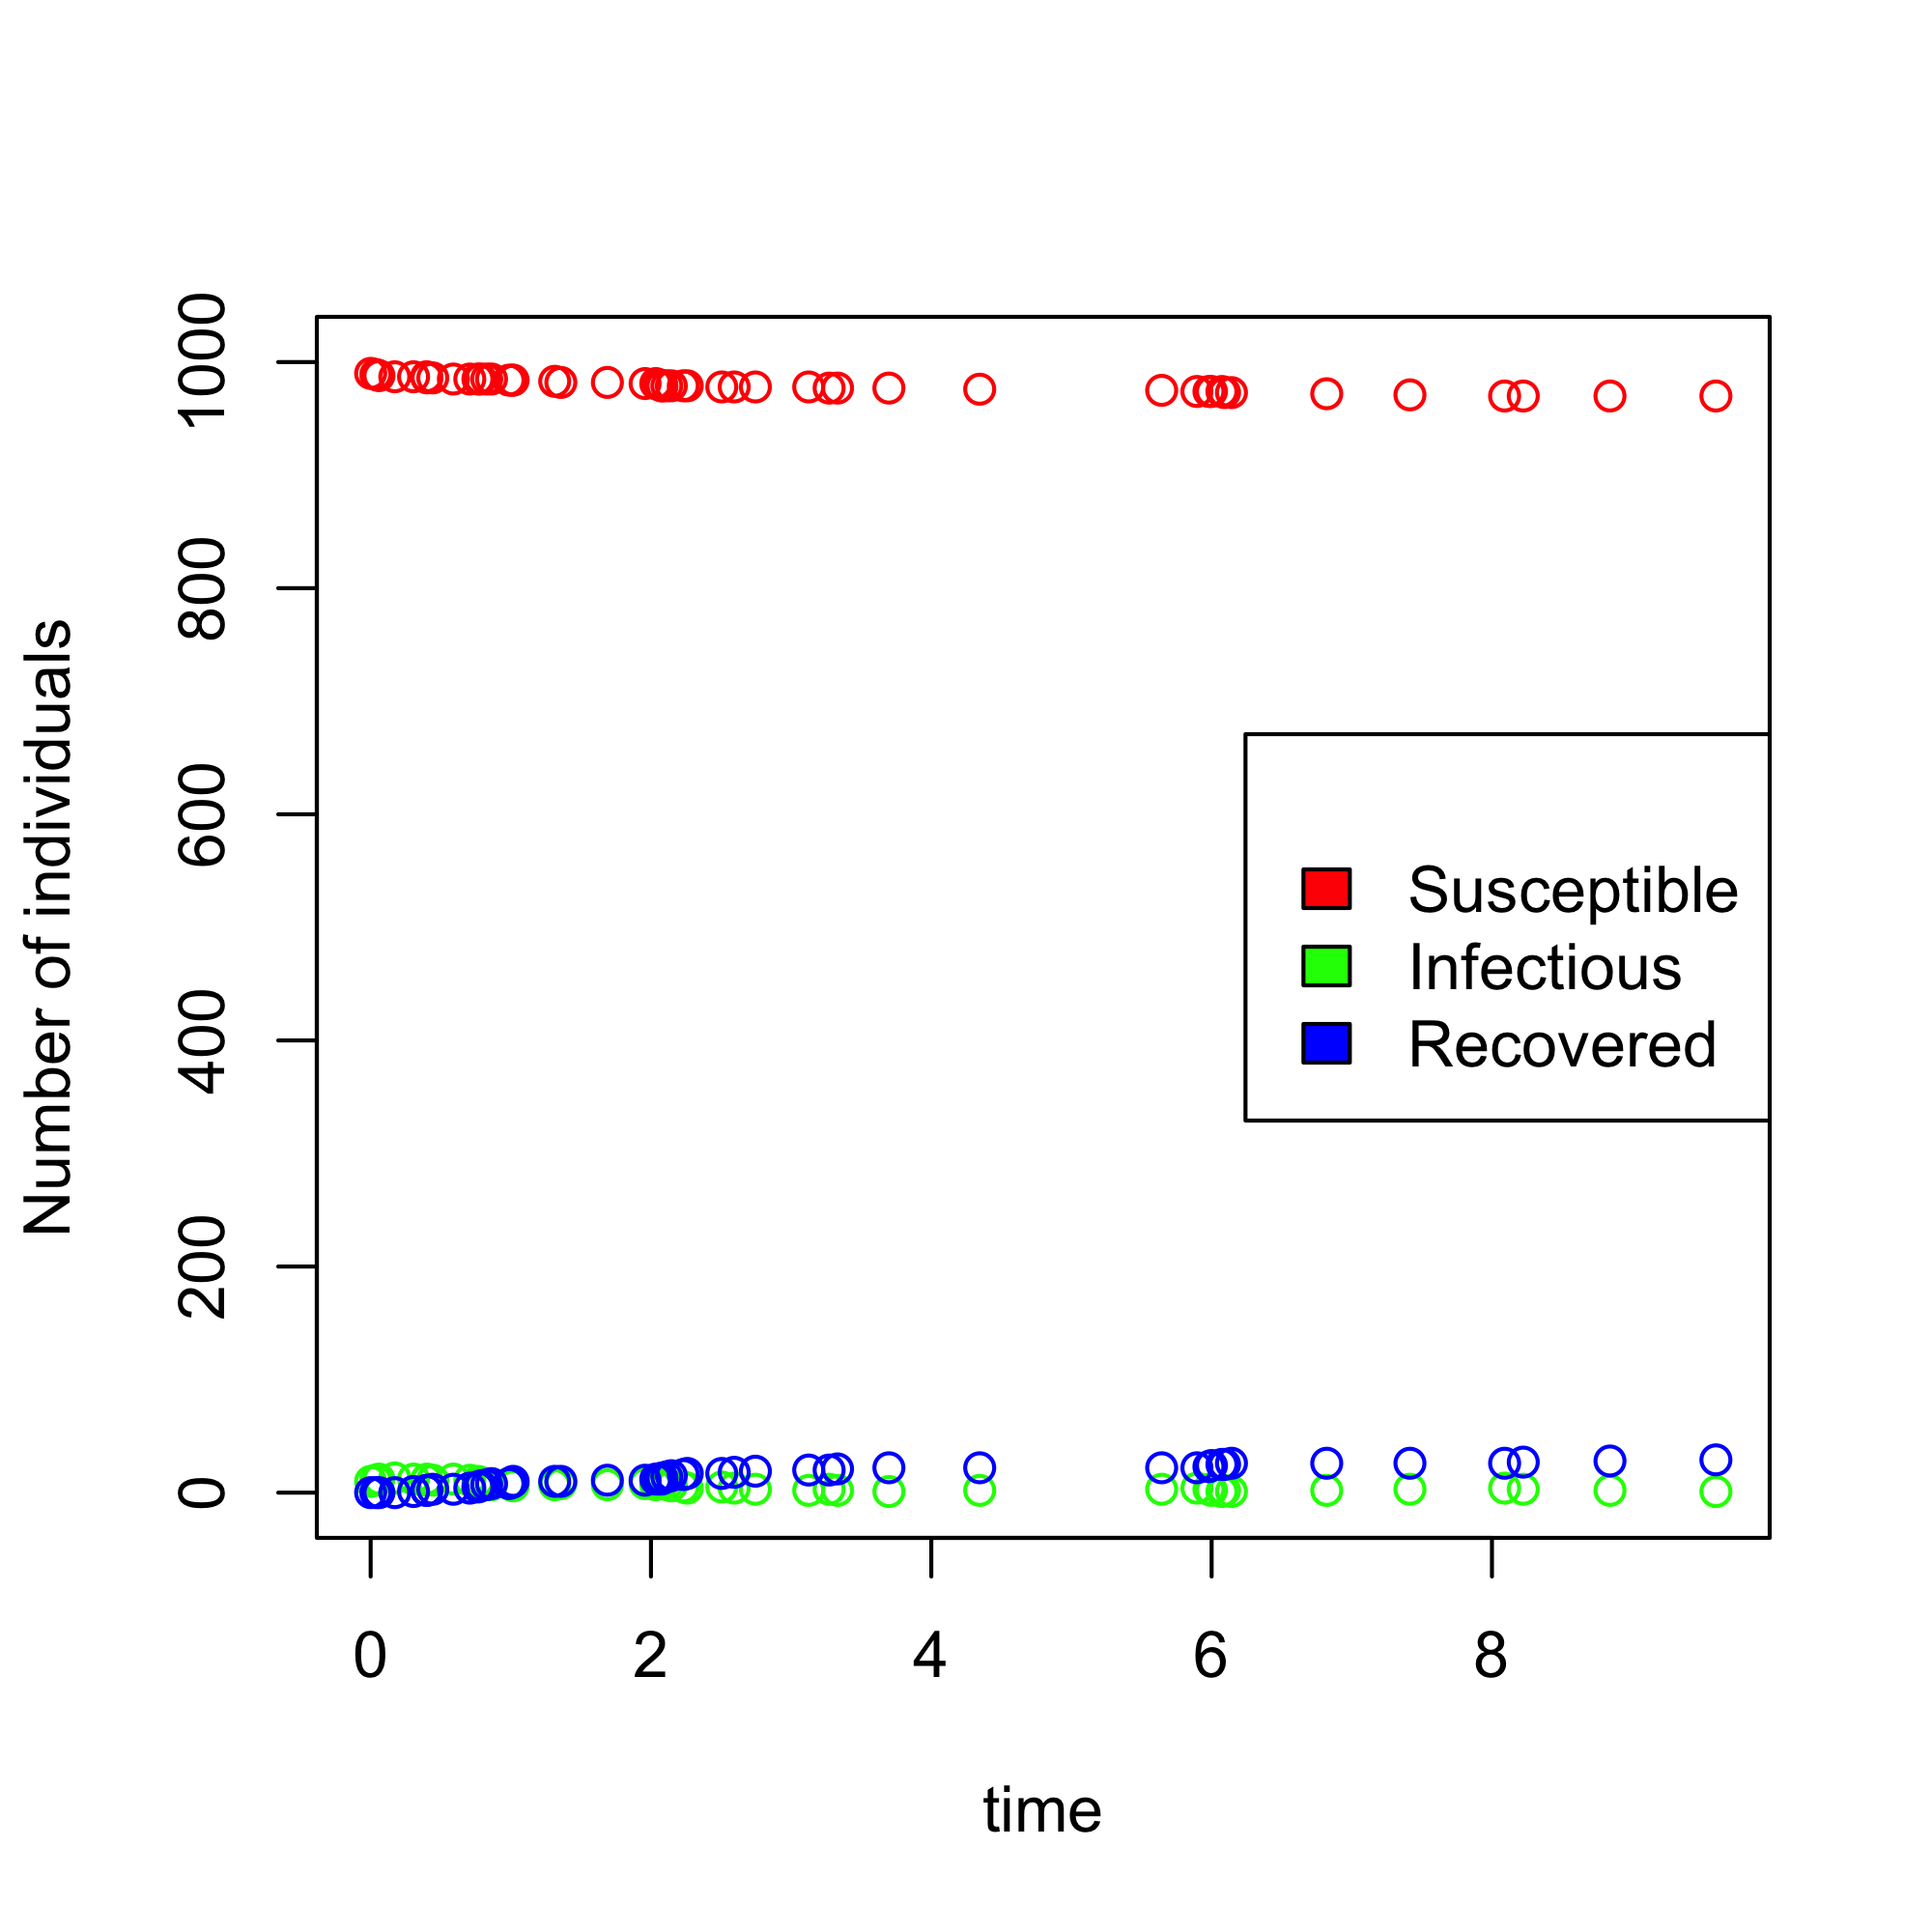
\includegraphics[width=\linewidth]{figures/trajectory_small_epidemic}
		\caption{Model with $R_0 = 0.5$.}
		\label{fig:trajectory_small_epidemic}
	\end{subfigure}
	\hfill
	\begin{subfigure}{0.45\linewidth}
		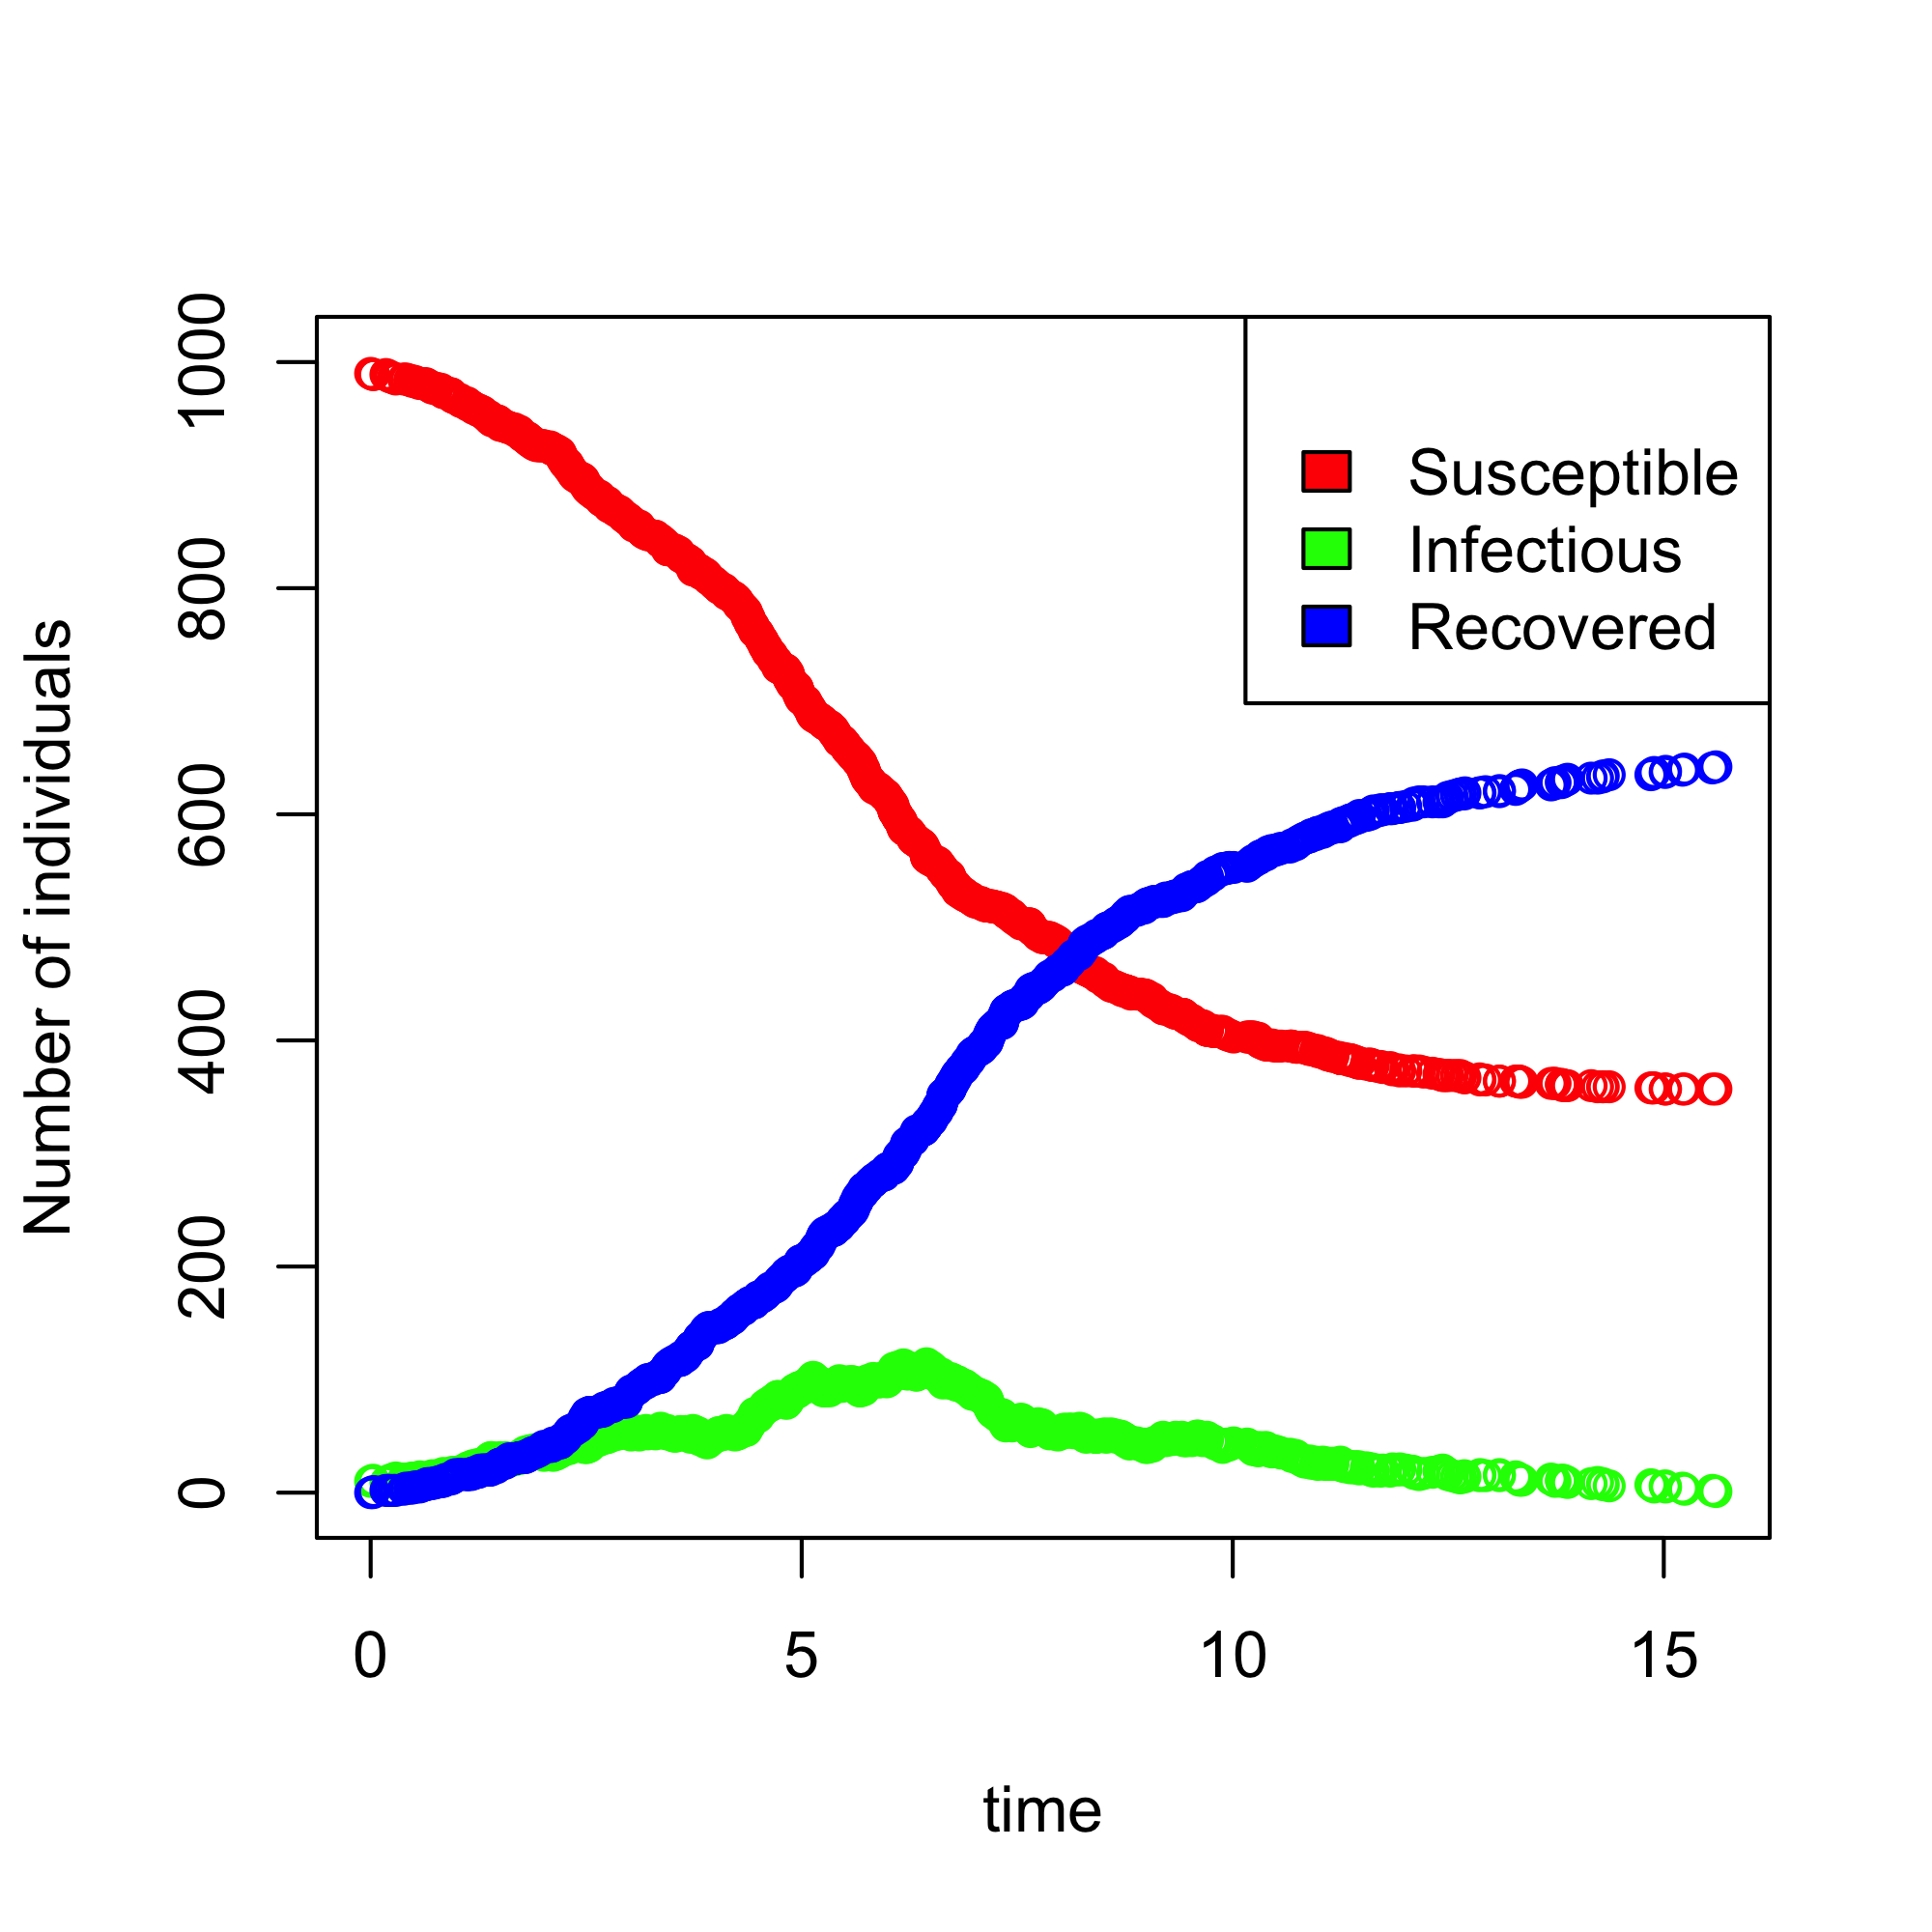
\includegraphics[width=\linewidth]{figures/trajectory_big_epidemic}
		\caption{Model with $R_0 = 1.5$.}
		\label{fig:trajectory_big_epidemic}
	\end{subfigure}
	\caption{Trajectories of a stochastic general epidemic model.} 
	\label{fig:trajectories}
\end{figure}

\begin{figure}
	\centering
	\begin{subfigure}{0.45\linewidth}
		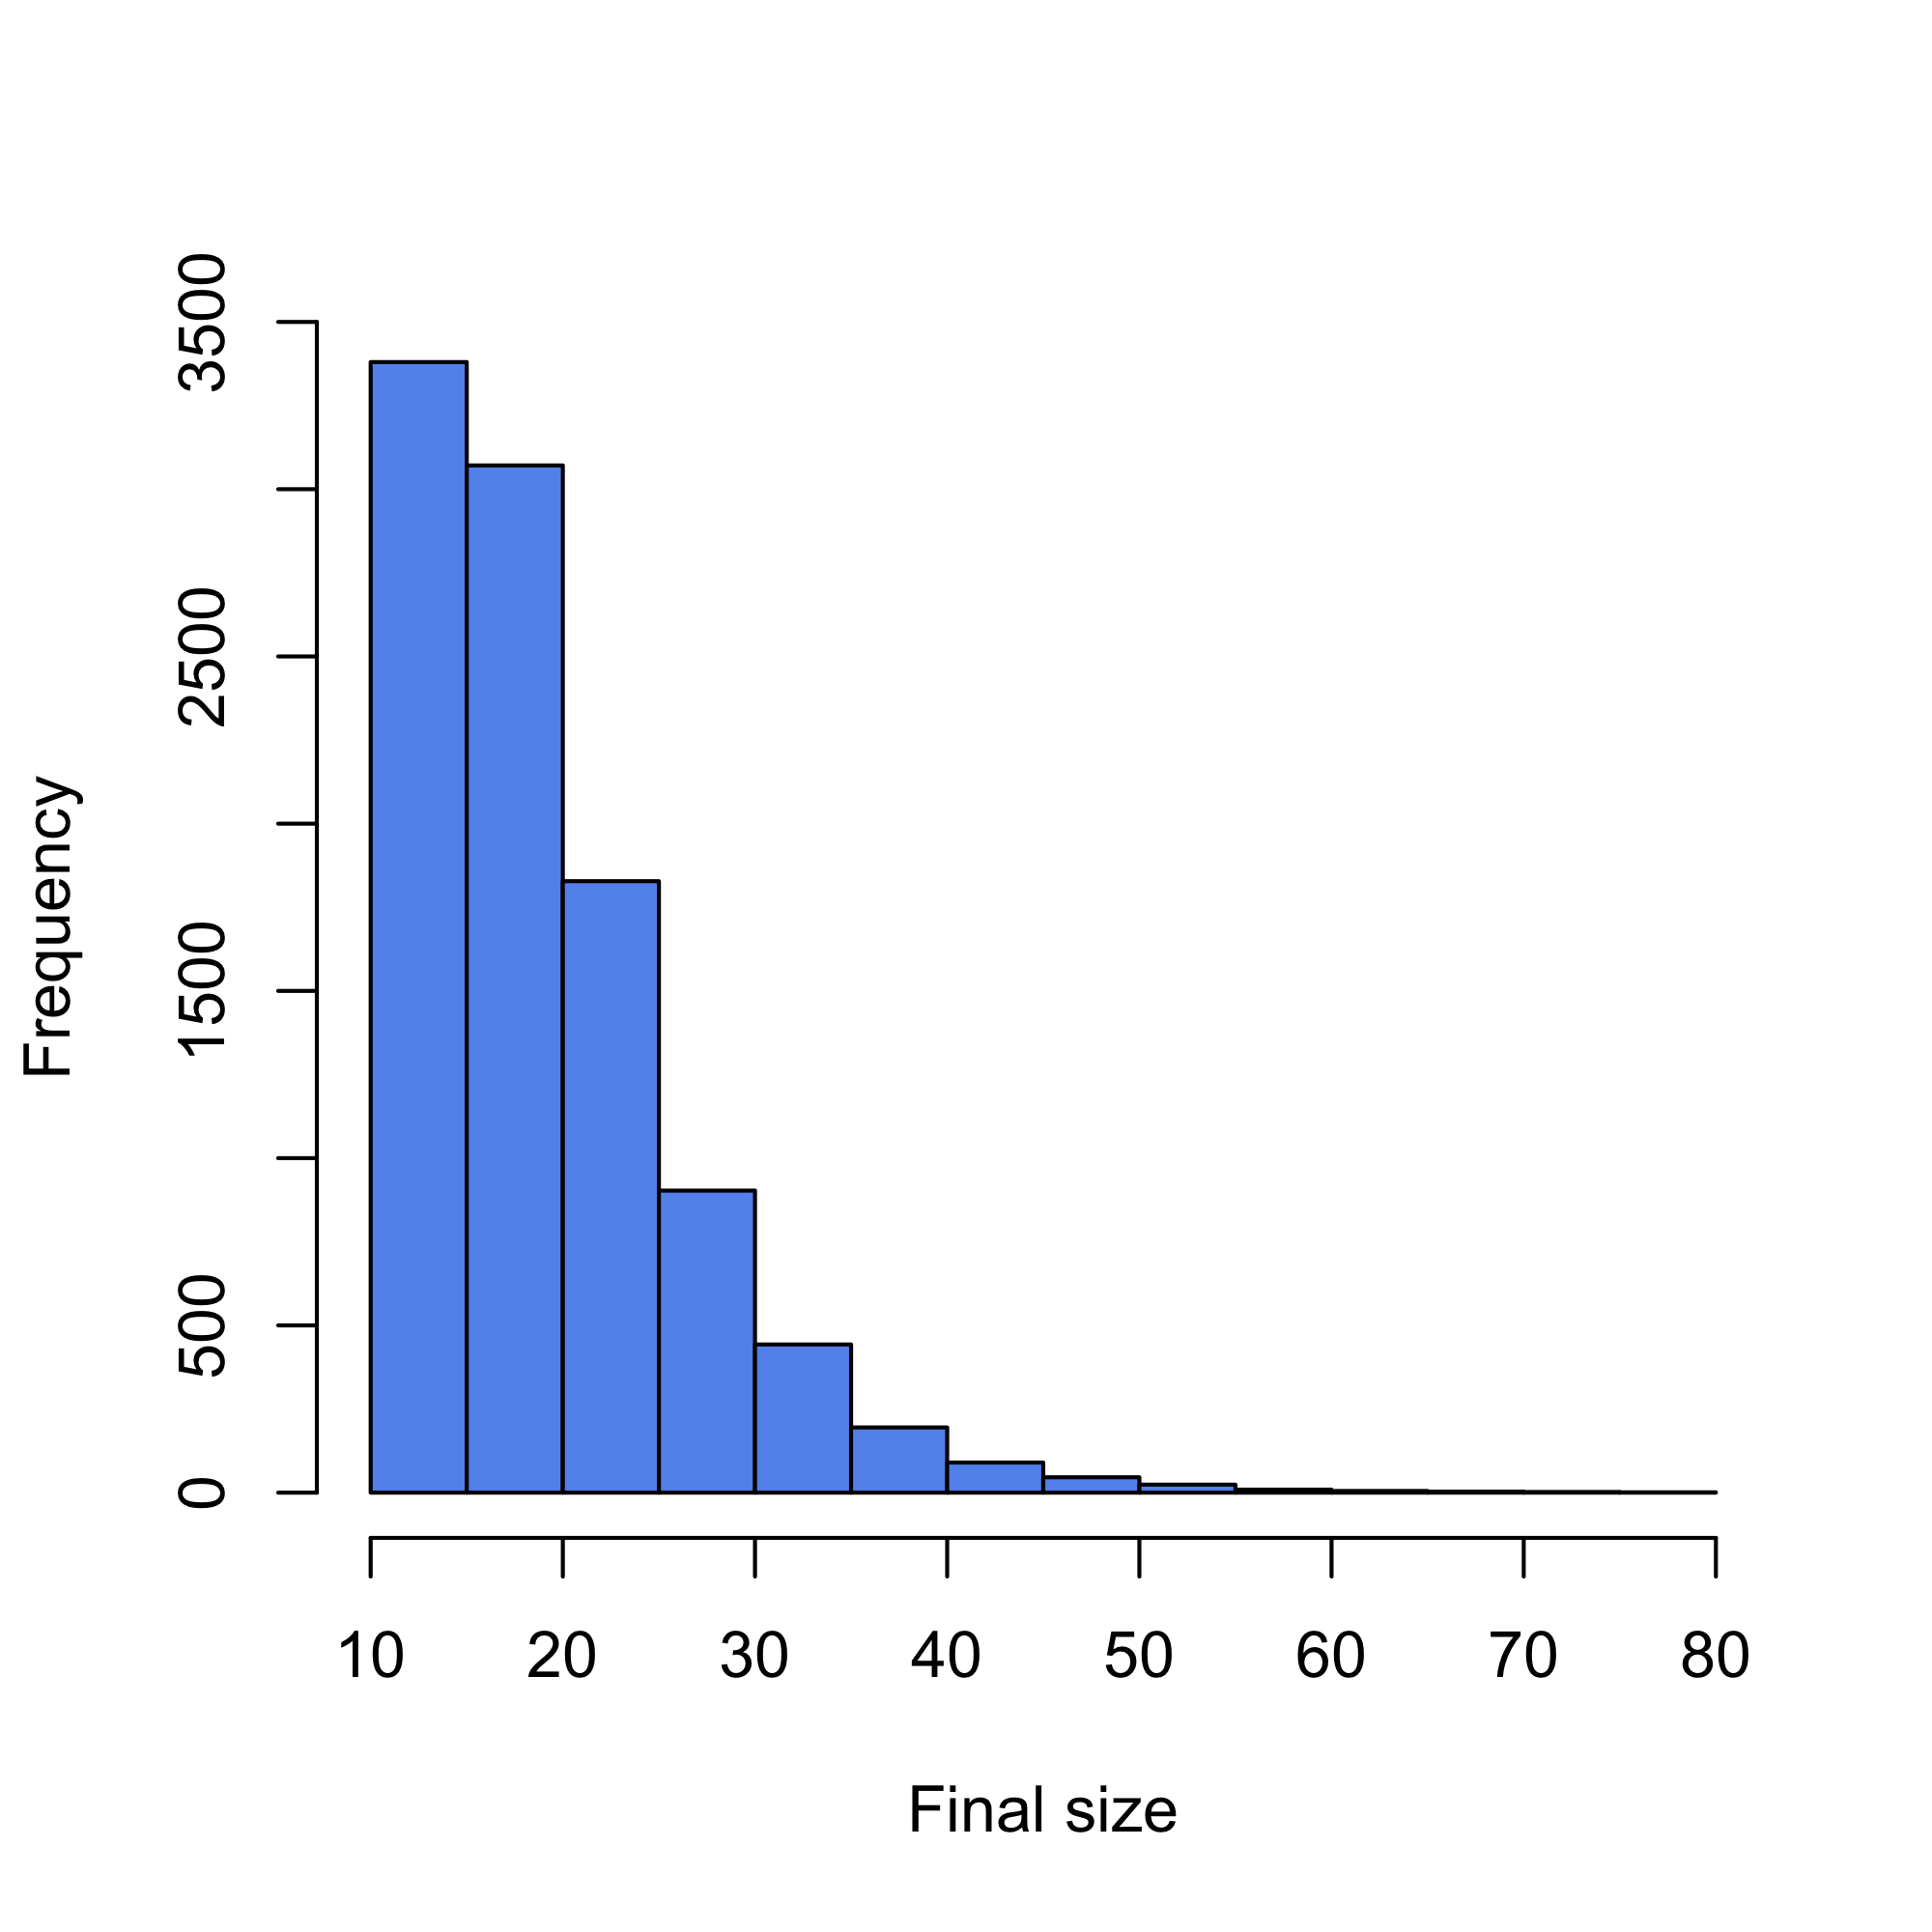
\includegraphics[width=\linewidth]{figures/final_size_small_epidemic}
		\caption{Final size distribution, $R_0 = 0.5$.}
		\label{fig:final_size_small_epidemic}
	\end{subfigure}
	\hfill
	\begin{subfigure}{0.45\linewidth}
		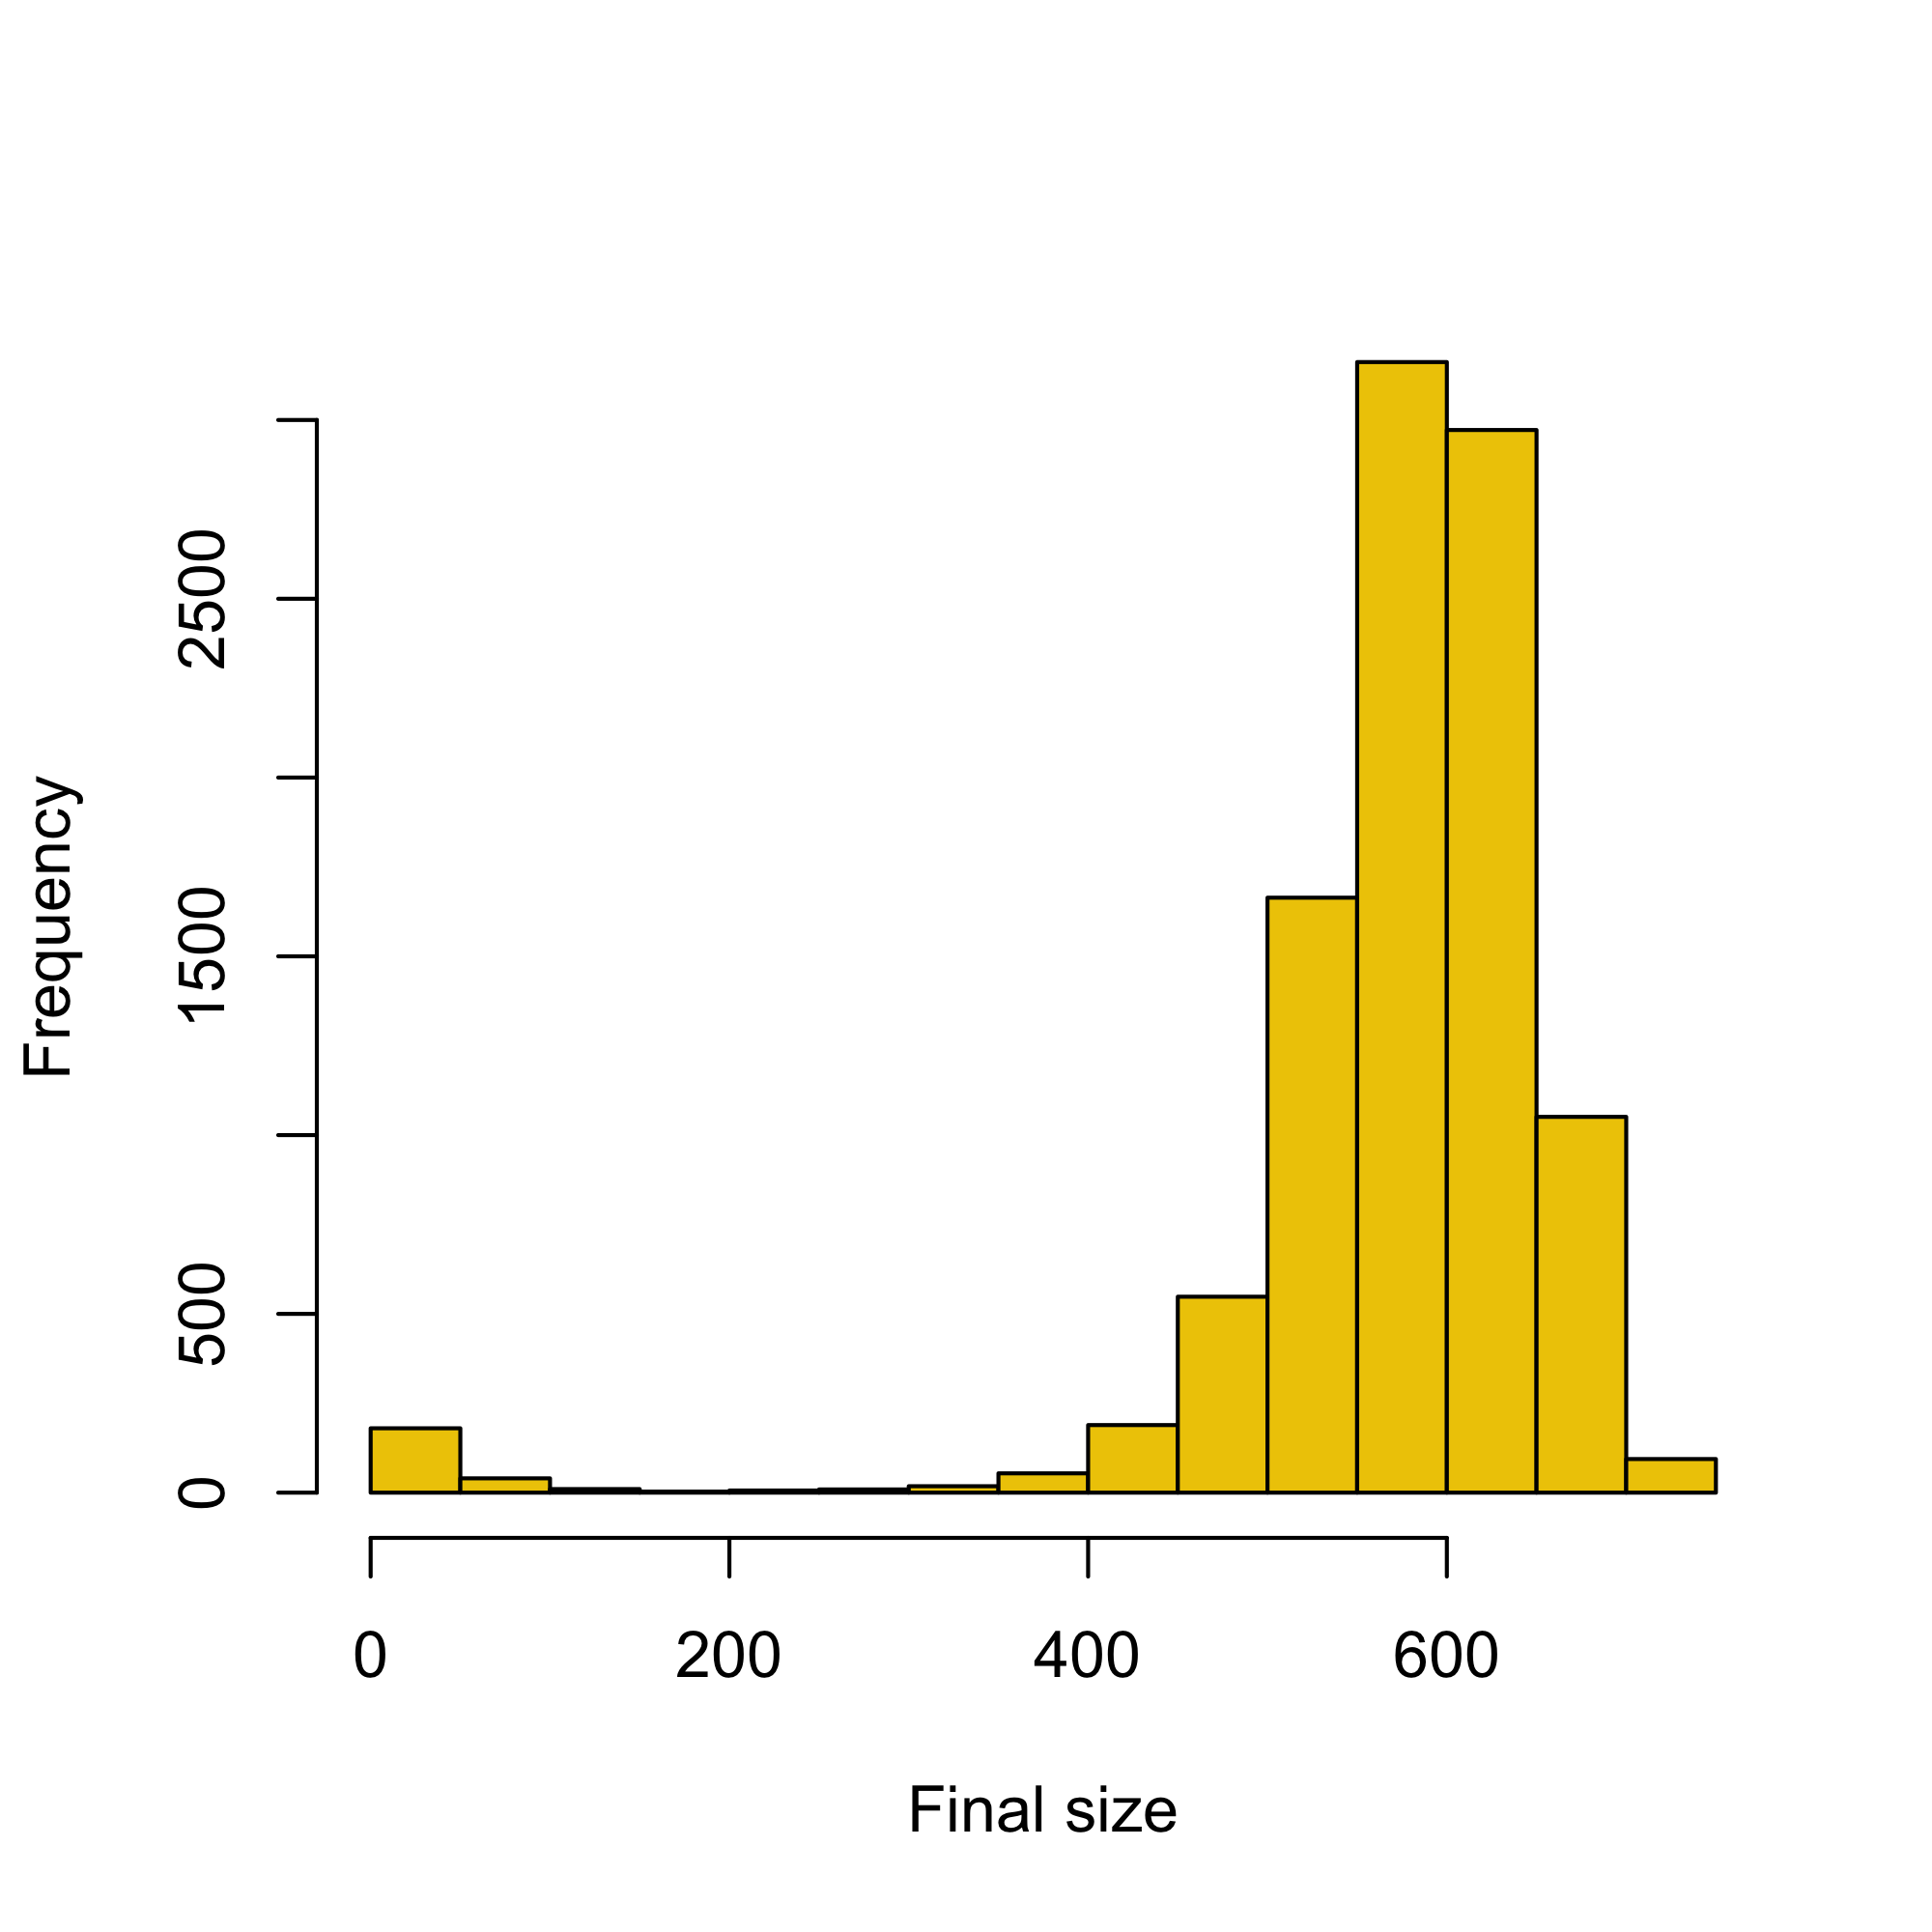
\includegraphics[width=\linewidth]{figures/final_size_big_epidemic}
		\caption{Final size distribution, $R_0 = 1.5$.}
		\label{fig:final_size_big_epidemic}
	\end{subfigure}
	\caption{Final size distribution of 10,000 simulations in a general stochastic epidemic model.} 
	\label{fig:final_size}
\end{figure}

\section{Network models}\label{sect:network}
One of the assumptions of the standard epidemic model, is that any two individuals have an equal probability of making contact. While this makes it simpler, it is of course less realistic. In reality, some people are more prone to being exposed (hospital or school workers, students), and more likely to infect those who are in close contact with them (coworkers, household members). A way to model this situations is to consider the members of the population as nodes in a network (see the book of \citet{Newman_2018} for basic network definitions). Such epidemic models abound in the scientific literature \citep{Deijfen_2011, Fransson_Trapman_2019, Kiss_Miller_Simon_2017, Pastor-Satorras-survey}. As an example, we define two such models, as they appear in the article of \citet{Britton_2019}. The interested reader is invited to read the survey by \citet{Pastor-Satorras-survey} or the work of \citet{Britton_2019}.

\begin{definition}[Discrete time Reed-Frost model on a network]
This model is a network generalization of the one described in Section \ref{sect:reedfrost}. Having an arbitrary network, a randomly chosen node is set as infectious at time $t = 0$, while the rest are susceptible. At time $t$, infectious individuals will infect susceptible neighbors (i.e., adjacent nodes) independently with probability $p$. The susceptible individuals that where infected at time $t$ will be infectious at time $t+1$, and infectious individuals at time $t$ will be removed at time $t+1$. This goes on until a time $T$ when there are no new infections.
\end{definition}


\begin{definition}[Continuous-time Markov chain model on a network]
	This model is a network generalization of the stochastic general epidemic model described in Section \ref{sect:standard_model}. Having an arbitrary network, a randomly chosen node is set as infectious at time $t = 0$, and the rest are susceptible. Infectious individuals have contacts with each susceptible neighbor (i.e. adjacent nodes) randomly in time according to an independent Poisson processes with rate $\lambda$ \citep{lawler_2006}. Each infected individual remains infectious for a period $I \sim \mathrm{Exp}(\gamma)$, after which it is removed from the epidemic (considered recovered and immune). Both infectious periods and contact processes are defined independently. This goes on until a time $T$ when there are no new infectious nodes.	
\end{definition}

As with the standard epidemic model in Section \ref{sect:standard_model}, the distribution of the infectious periods can be chosen arbitrarily, at the expense of the Markovian property. Similarly, setting a constant infectious period gives rise to a continuous-time Reed-Frost model \citep{Britton_2019}.


\section{COVID-19 pandemic}\label{sect:covid}
At the moment this work is being written, a pandemic caused by the SARS-CoV-2, colloquially known as COVID-19, is widespread in most countries of the world. Various authors have tried to estimate this disease's $R_0$; a review by \citet{Liu_Gayle_2020} has found that the mean $R_0$ estimated is of 3.28, with a median of 2.79. In the Mexican northern state of Nuevo León, the first cases were reported in March 2020. In Figure \ref{fig:nl}, two graphics are shown regarding the spread of the epidemic process in Nuevo León from April 1st, 2020 to November 30th, 2020, with information provided by the Mexican government \citep{datos_covid}. In particular, a graph of the cumulative cases in the state is shown in Figure \ref{fig:nl_cum}. A 7-day rolling average of cases per day is seen in Figure \ref{fig:nl_roll}. In a stochastic general epidemic model, as the presented in Section \ref{sect:standard_model}, an $R_0$ of 3 would give a limiting fraction of .94 infected in the population, by solving Equation \ref{eq:limiting_fraction}. This can be seen in the trajectory in Figure \ref{fig:trajectory_r03_epidemic}, a simulated trajectory of an epidemic in a population of 1000 which has $R_0 = 3$. This of course should not be interpreted as a suggestion that the current pandemic will infect 94\% of the population, since the model is quite weak in its assumptions. It is, however, a simplified example of how quickly these processes can grow out of control when there is nothing stopping its spread.


\begin{figure}
	\centering
	\begin{subfigure}{0.45\linewidth}
		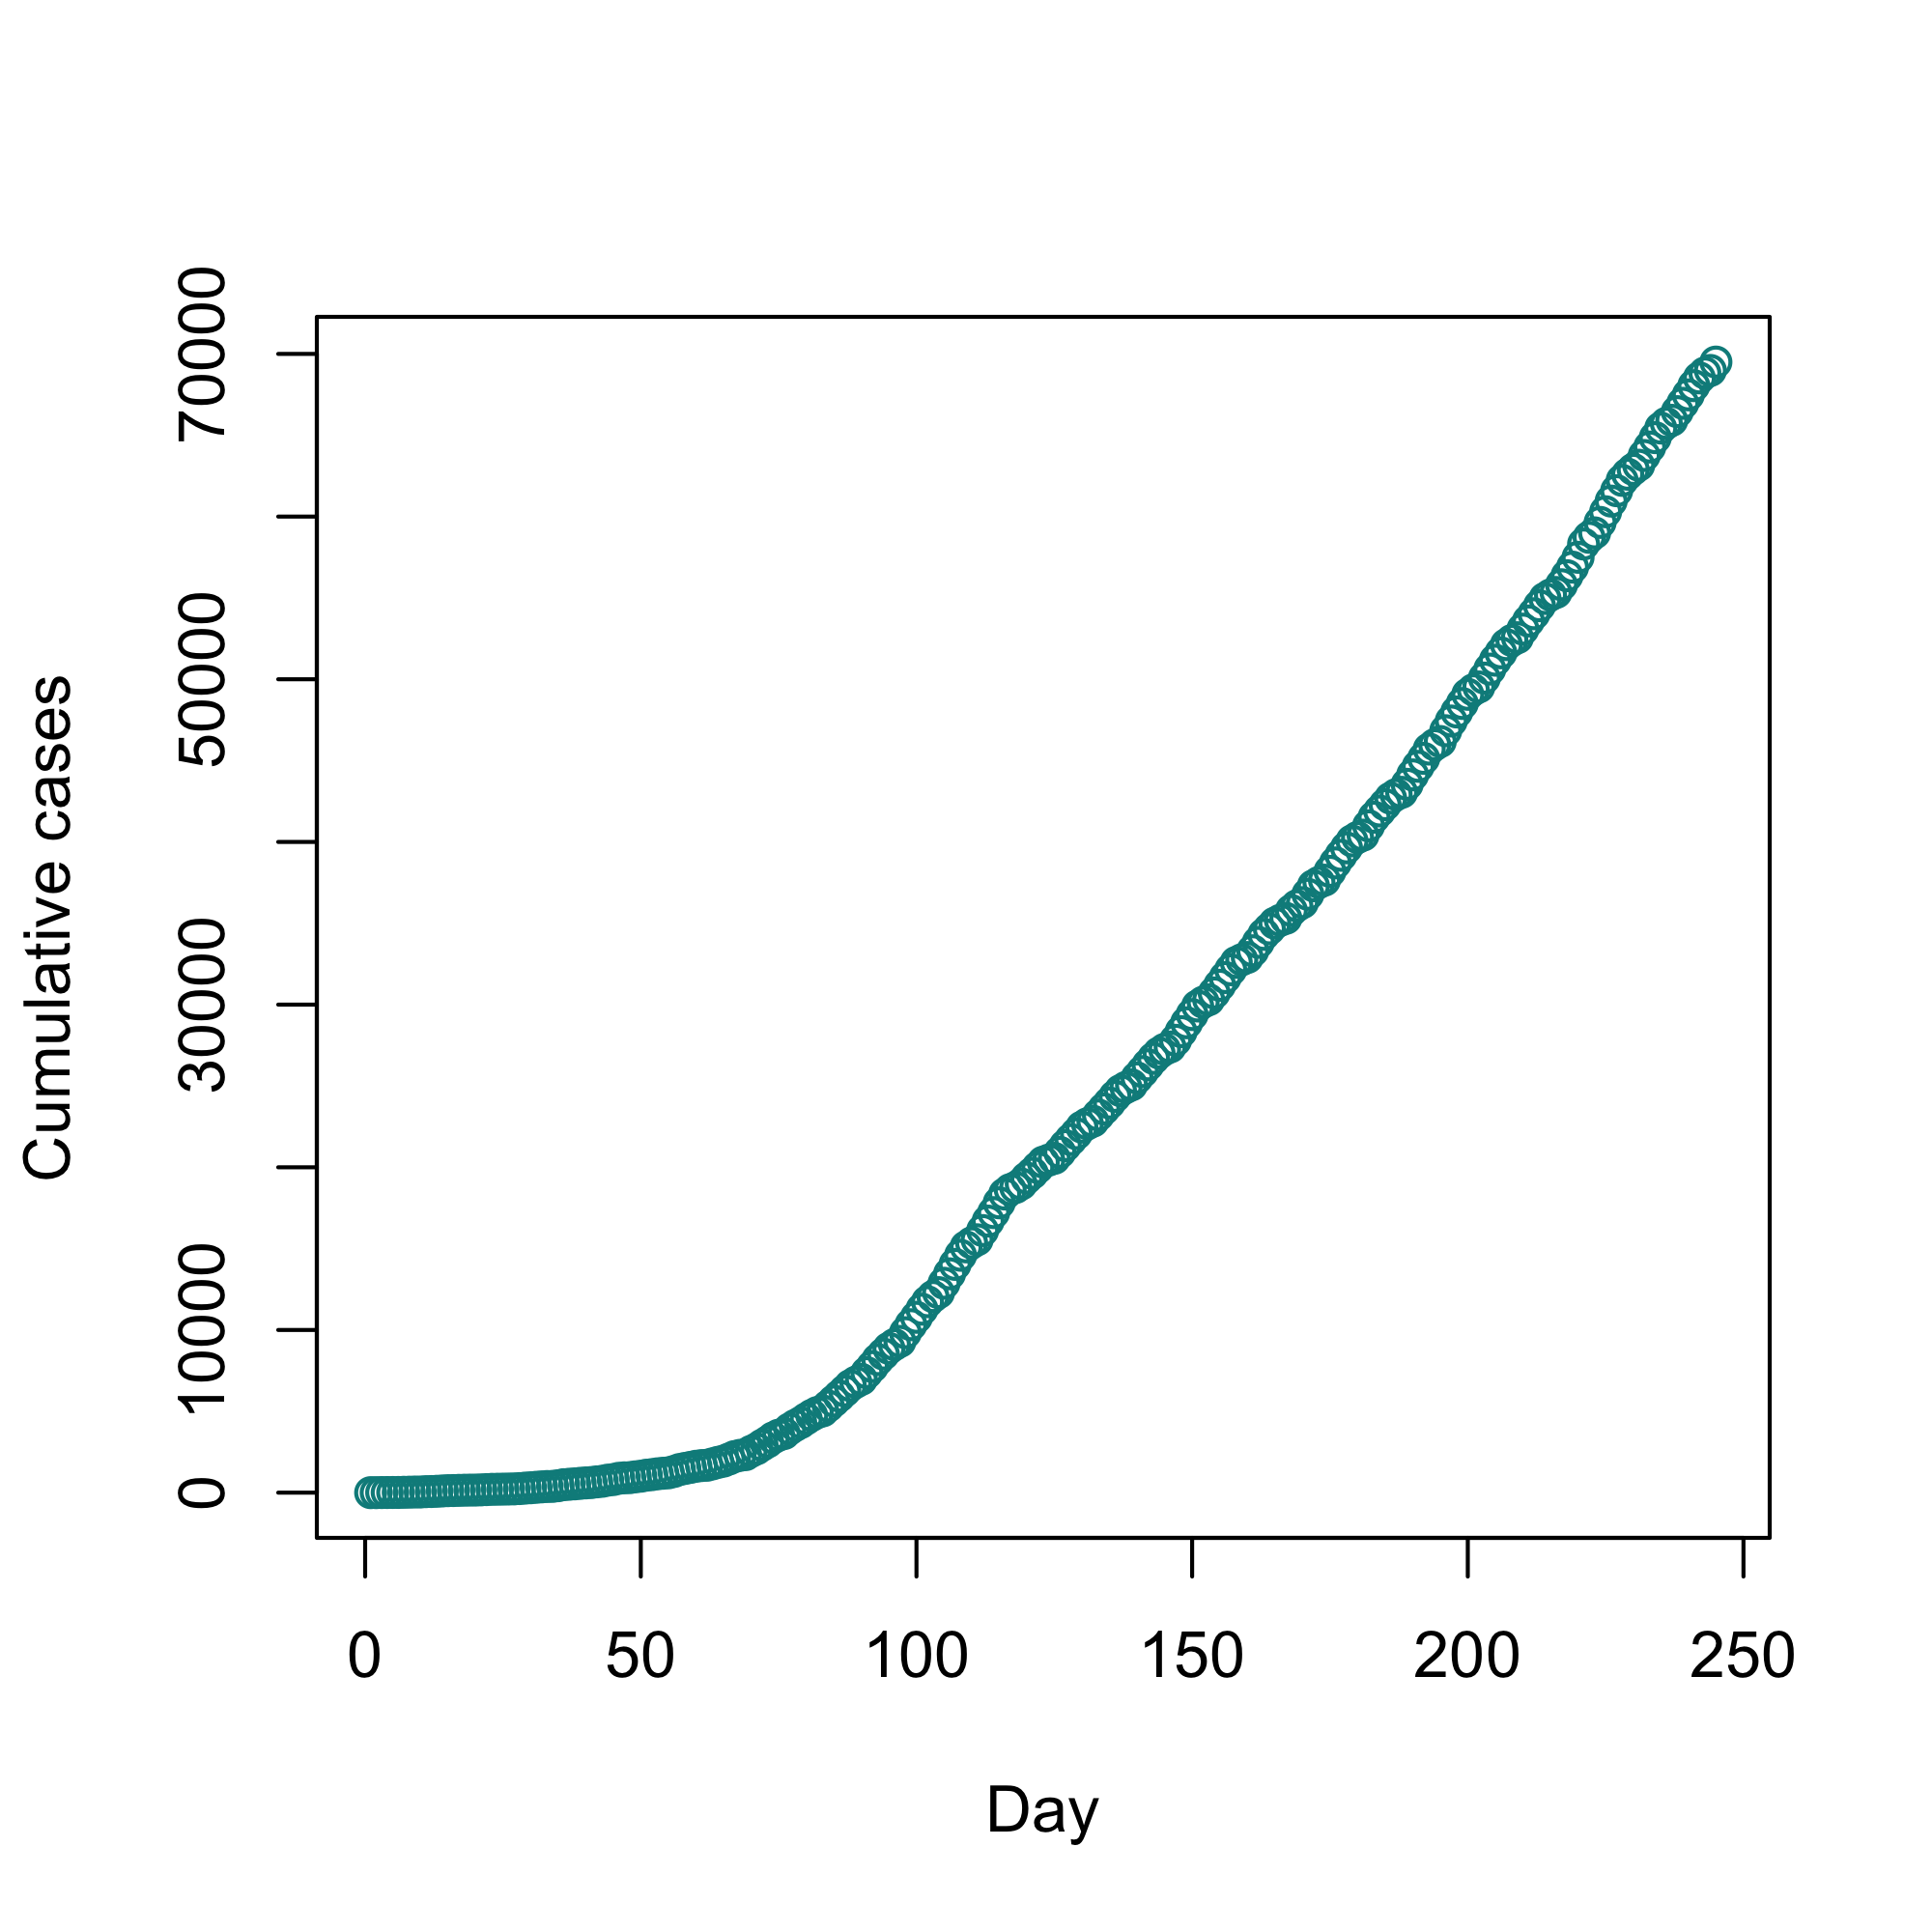
\includegraphics[width=\linewidth]{figures/nl_cumulative}
		\caption{Cumulative COVID-19 cases in Nuevo León.}
		\label{fig:nl_cum}
	\end{subfigure}
	\hfill
	\begin{subfigure}{0.45\linewidth}
		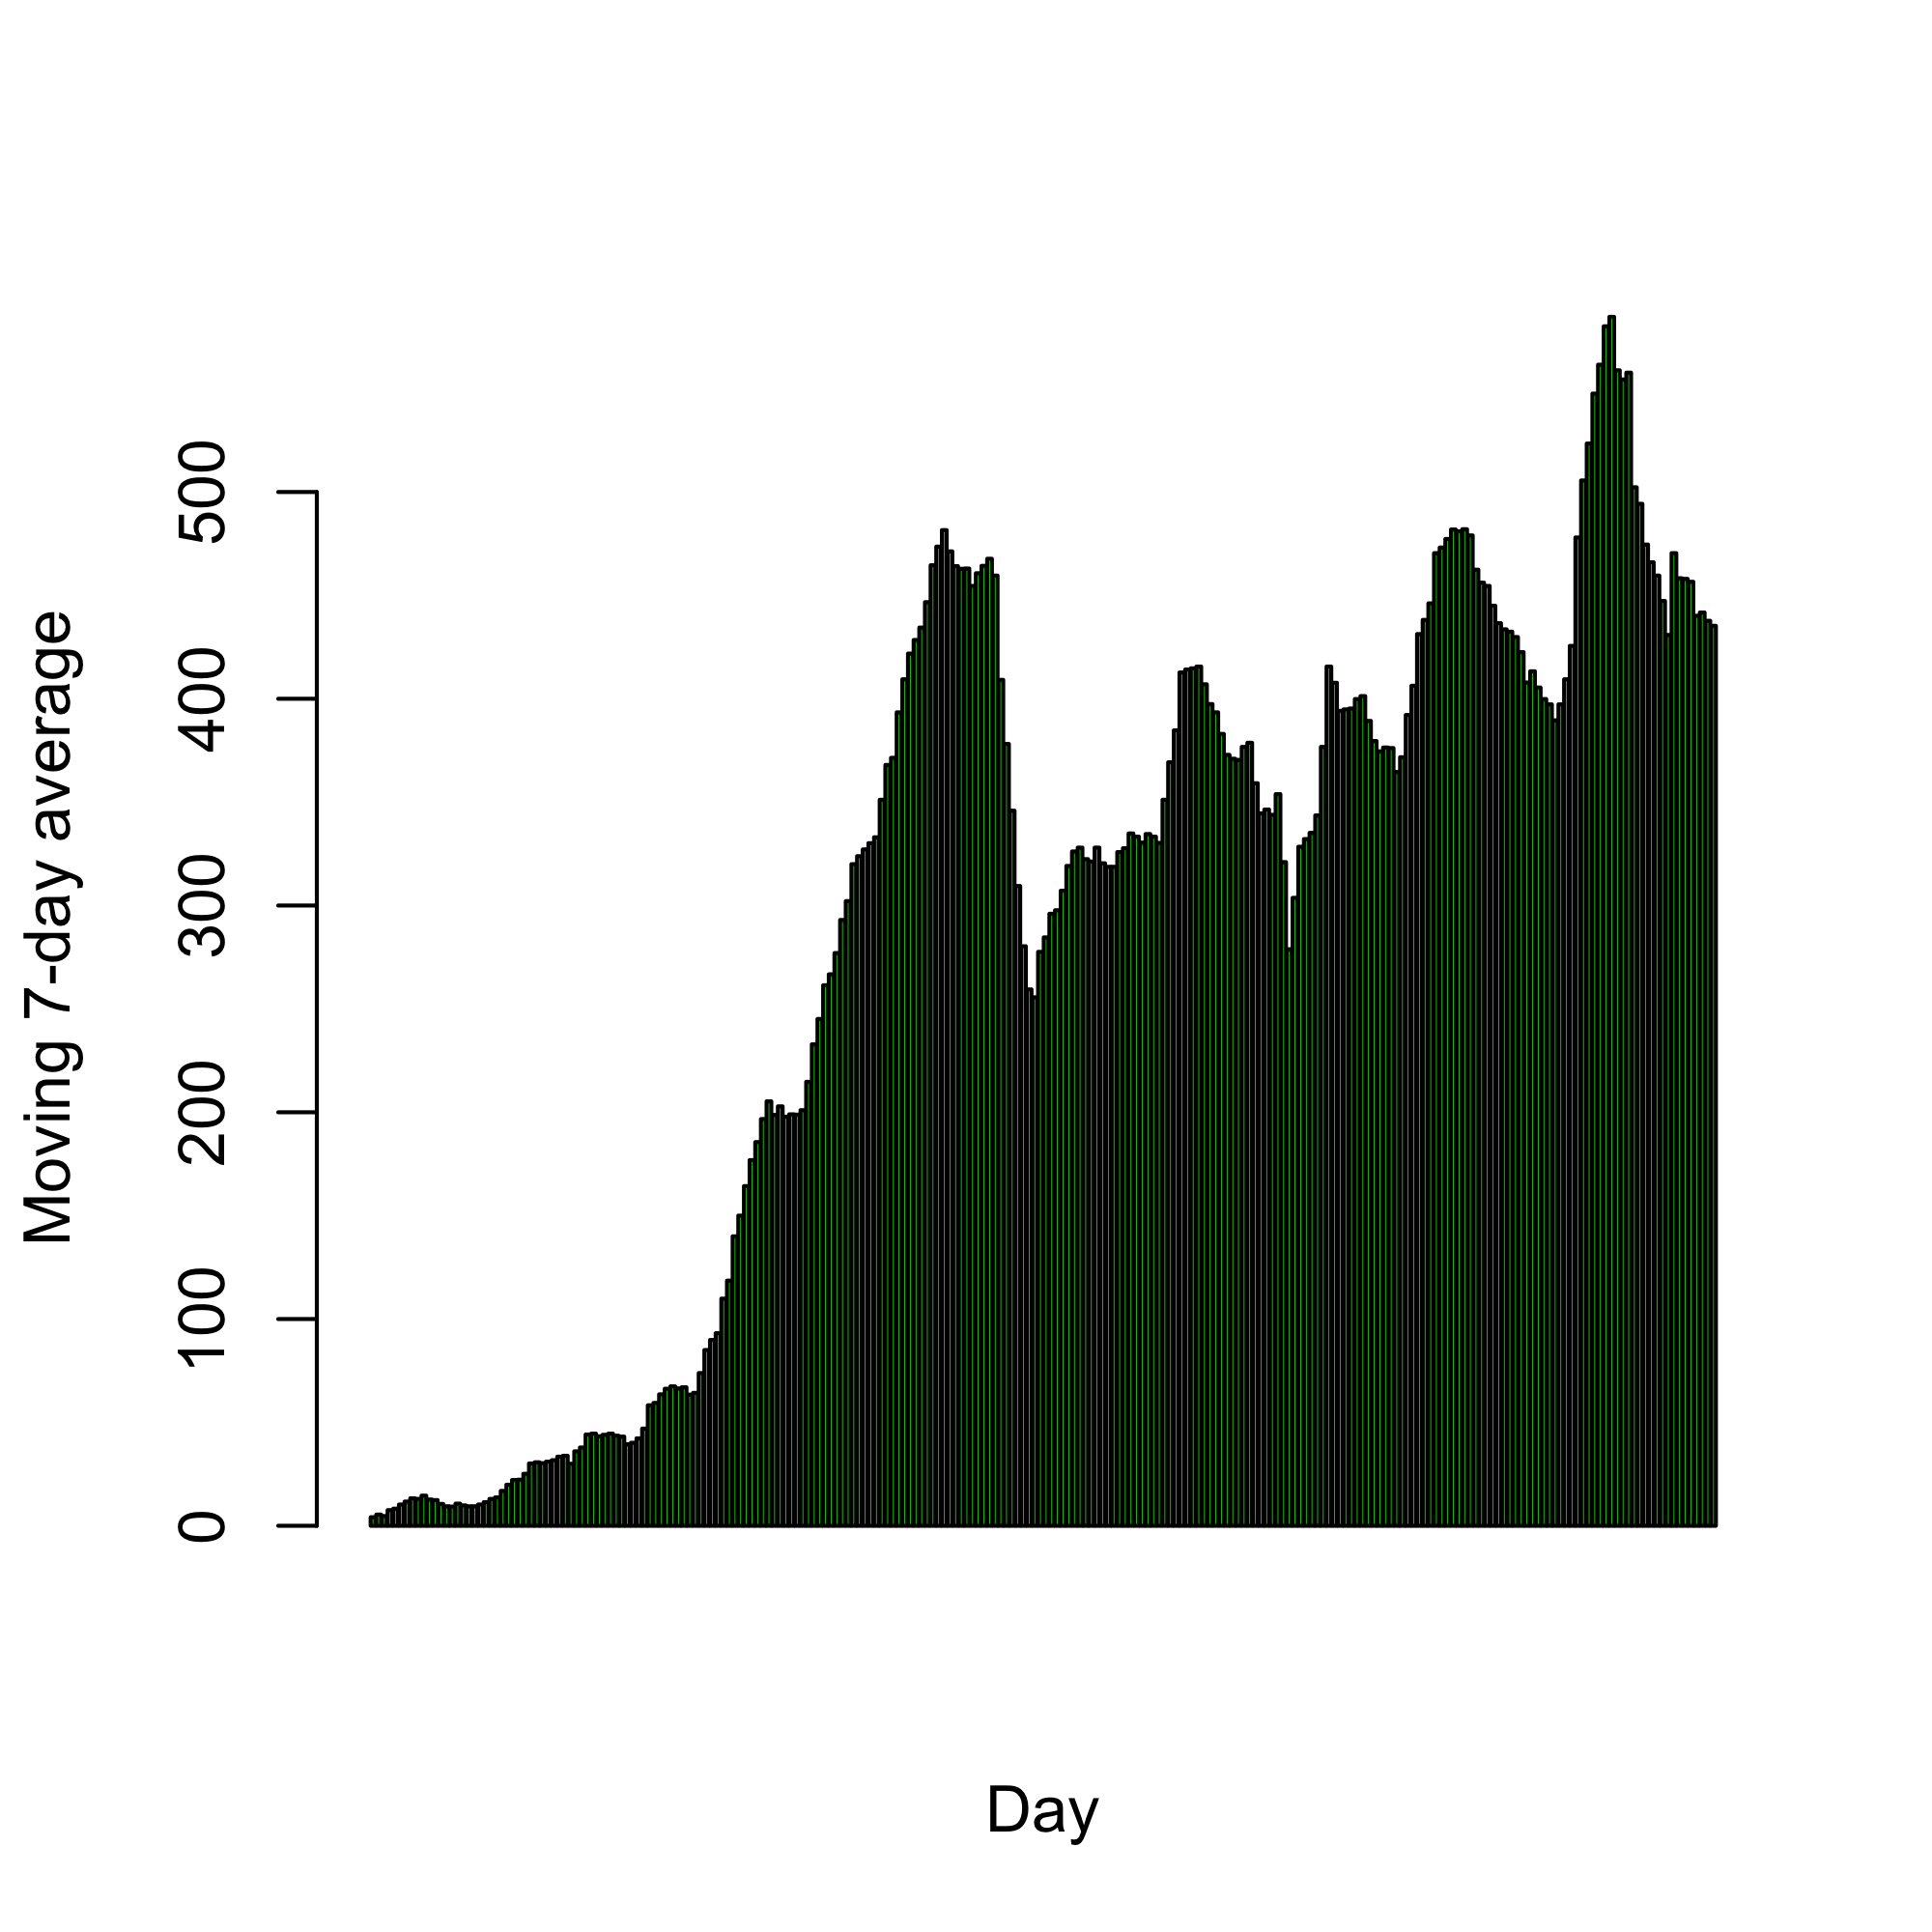
\includegraphics[width=\linewidth]{figures/roll_average_nl}
		\caption{Rolling 7-day average of COVID-19 cases in Nuevo León.}
		\label{fig:nl_roll}
	\end{subfigure}
	\caption{COVID-19 cases in the state of Nuevo León from 2020-04-01 to 2020-11-30.} 
	\label{fig:nl}
\end{figure}

\begin{figure}
\centering
	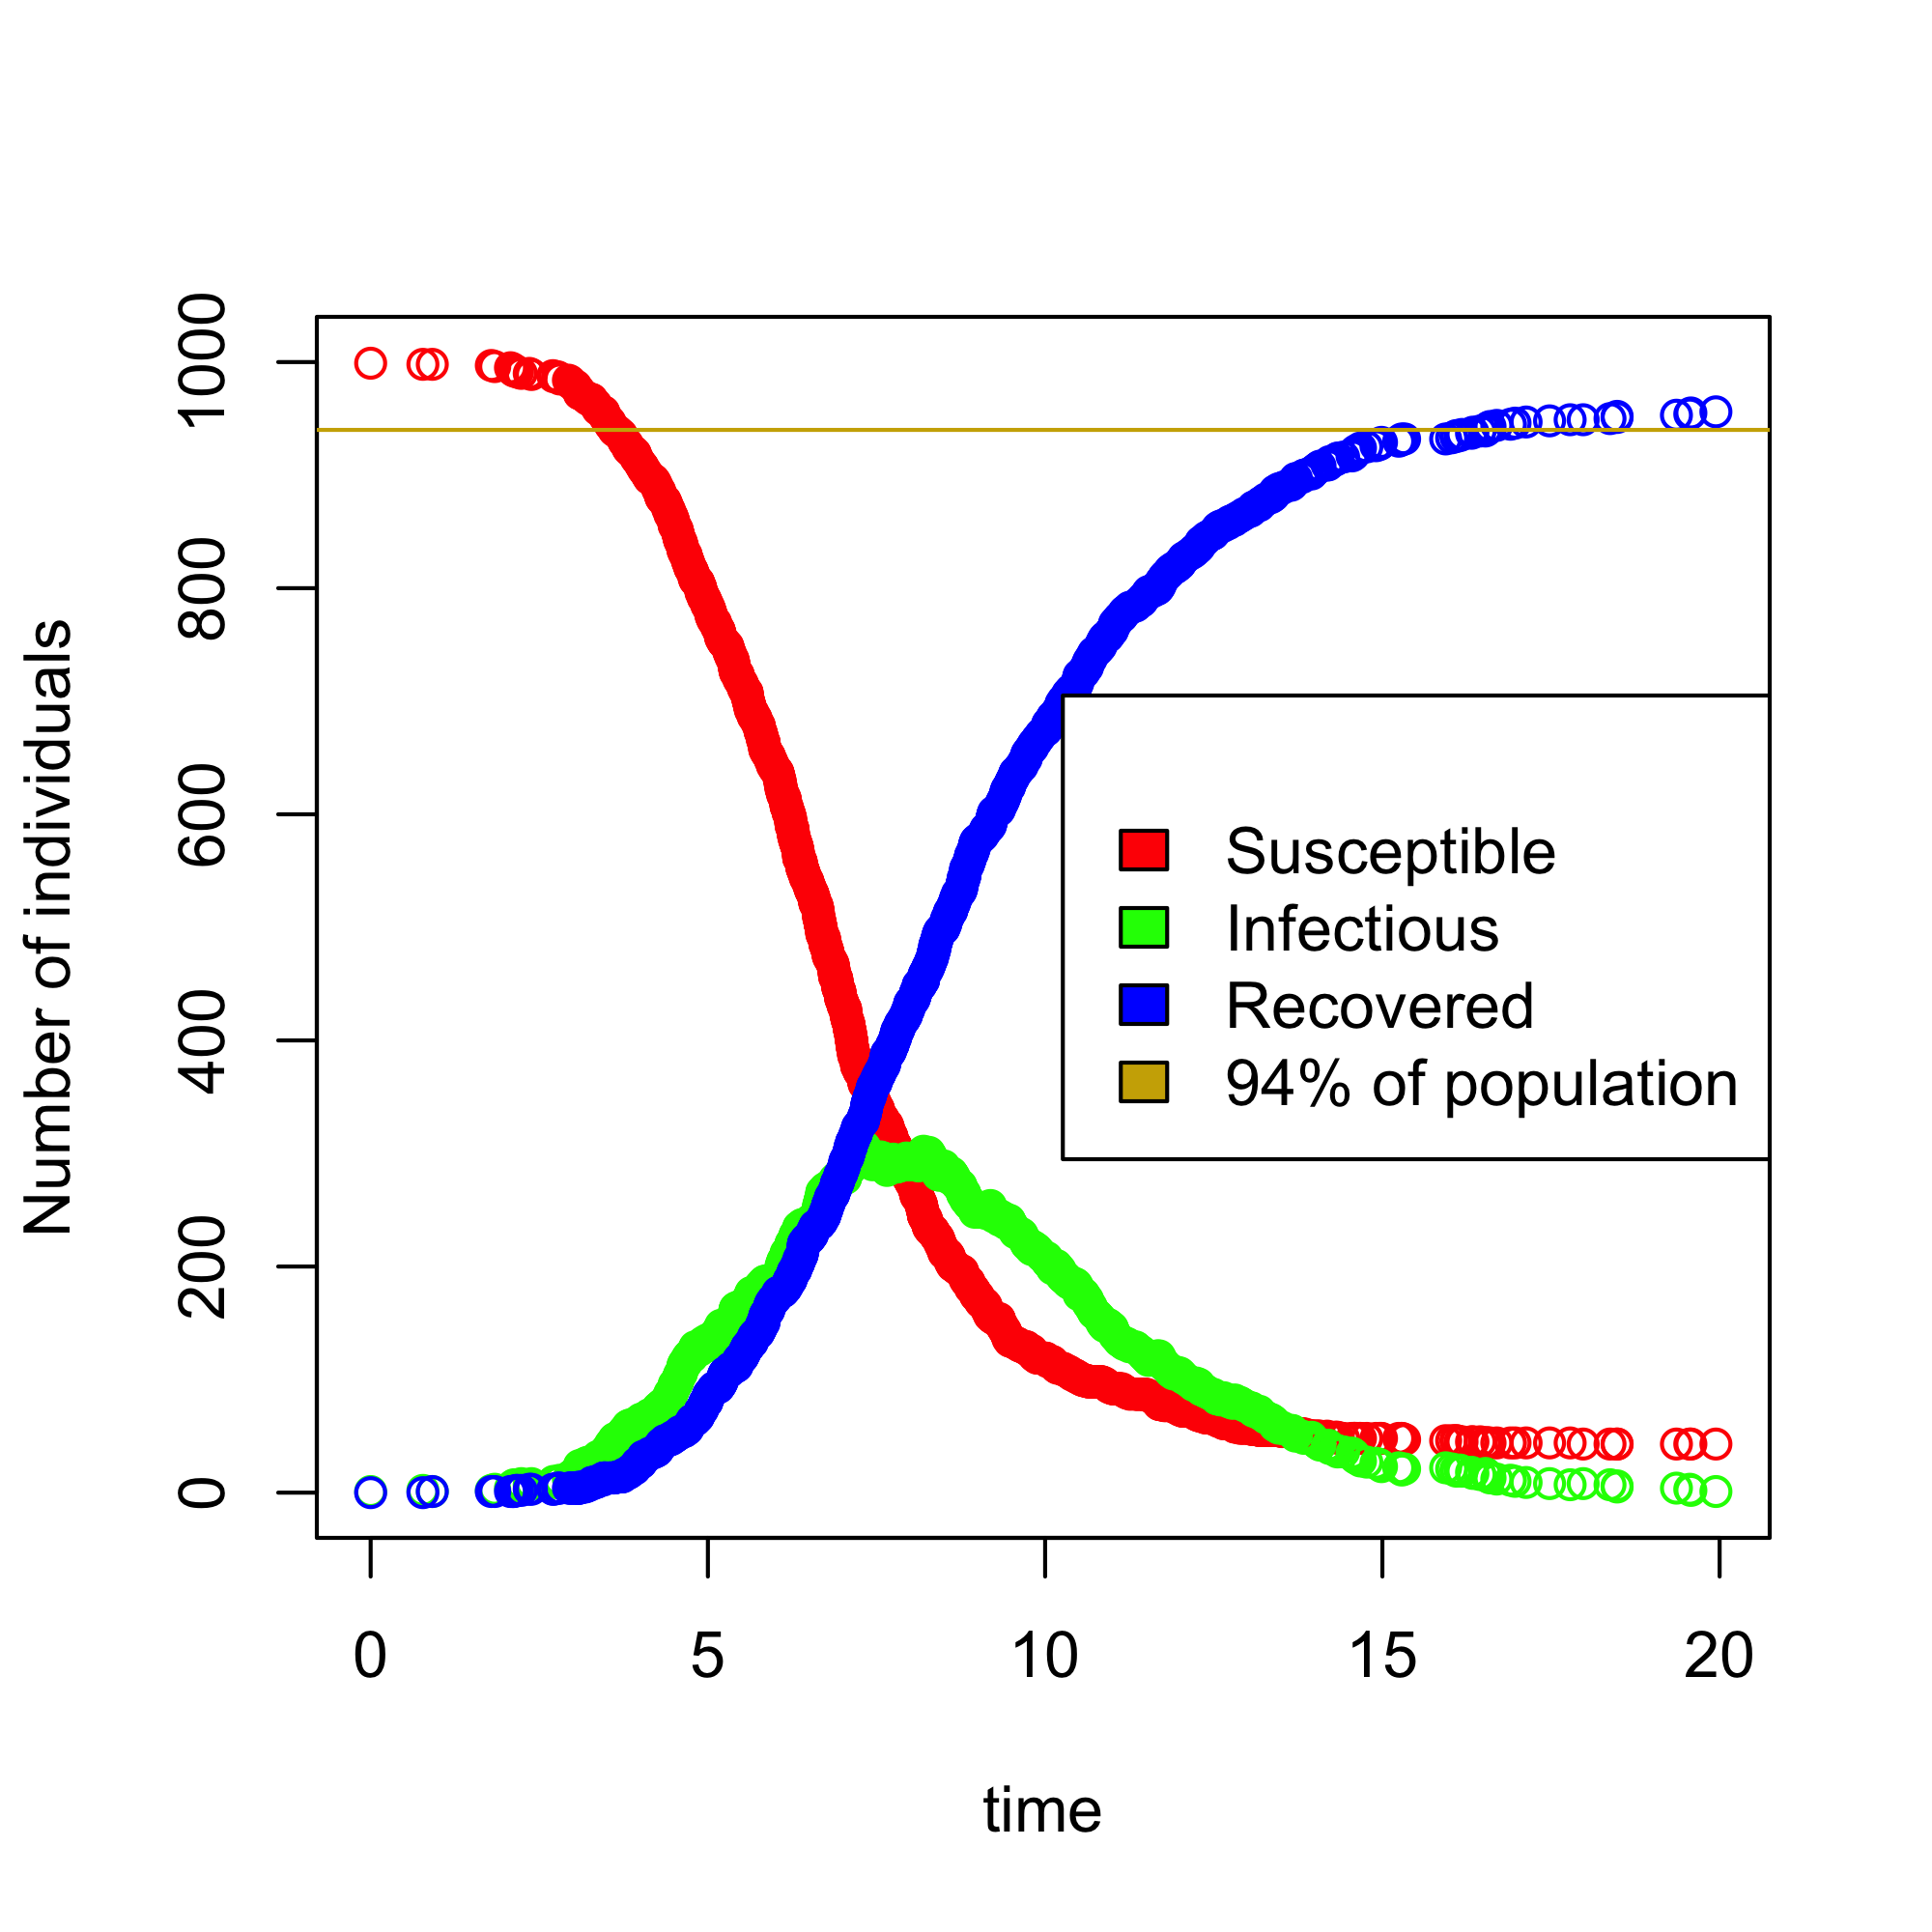
\includegraphics[width=.5\linewidth]{figures/trajectory_r0_3}
	\caption{General stochastic model with $R_0 = 3$.}
	\label{fig:trajectory_r03_epidemic}
\end{figure}

\section{Conclusions}\label{sect:conclusions}
In this work, two common epidemic models were presented, as well as generalizations to network models. In particular, the standard stochastic epidemic model was studied in more detail. Simulations were performed and displayed. Finally, some discussion of how these relate to a current, ongoing pandemic was presented. The standard stochastic epidemic model can be generalized beyond its SIR presentation. Models for further study include those were there is an incubation period after infection, before becoming infectious (SEIR) or those with waning immunity (SIRS). Models with dynamic population, taking into account births and deaths or migration, were also lacking in this work. While the network models in Section \ref{sect:network} remove the well-mixed assumption of the population, individuals are still homogeneous. Multi-type models \citep{Andersson_Britton_2000} address this limitations, and can be studied in further work. 
%%%%%%%%%%%%%%%%%%%%%%%%%%%%%%%%%%%%%%%%%%%%%%
%% Support information (funding), if any,   %%
%% should be provided in the                %%
%% Acknowledgements section.                %%
%%%%%%%%%%%%%%%%%%%%%%%%%%%%%%%%%%%%%%%%%%%%%%
\section*{Acknowledgements}
The author thanks the financial support of CONACyT, and the suggestion of Fabiola V\'azquez to incorporate in this work data from a real epidemic.


%%%%%%%%%%%%%%%%%%%%%%%%%%%%%%%%%%%%%%%%%%%%%%
%% Supplementary Material, if any, should   %%
%% be provided in {supplement} environment  %%
%% with title and short description.        %%
%%%%%%%%%%%%%%%%%%%%%%%%%%%%%%%%%%%%%%%%%%%%%%
%\begin{supplement}
%\stitle{Title of Supplement A}
%\sdescription{Short description of Supplement A.}
%\end{supplement}
%\begin{supplement}
%\stitle{Title of Supplement B}
%\sdescription{Short description of Supplement B.}
%\end{supplement}

%%%%%%%%%%%%%%%%%%%%%%%%%%%%%%%%%%%%%%%%%%%%%%%%%%%%%%%%%%%%%
%%                  The Bibliography                       %%
%%                                                         %%
%%  imsart-???.bst  will be used to                        %%
%%  create a .BBL file for submission.                     %%
%%                                                         %%
%%  Note that the displayed Bibliography will not          %%
%%  necessarily be rendered by Latex exactly as specified  %%
%%  in the online Instructions for Authors.                %%
%%                                                         %%
%%  MR numbers will be added by VTeX.                      %%
%%                                                         %%
%%  Use \cite{...} to cite references in text.             %%
%%                                                         %%
%%%%%%%%%%%%%%%%%%%%%%%%%%%%%%%%%%%%%%%%%%%%%%%%%%%%%%%%%%%%%

%% if your bibliography is in bibtex format, uncomment commands:
\bibliographystyle{imsart-nameyear} % Style BST file (imsart-number.bst or imsart-nameyear.bst)
\bibliography{ref}       % Bibliography file (usually '*.bib')

\end{document}
